\section{Pipeline ETL (Apache Airflow)}
\label{chap:etl}
Cette section décrit le pipeline qui alimente la plateforme à partir des fichiers tableurs historiques de SOYAFF. Il réalise les exigences \texttt{EF-ETL-01} (import de l'historique) et \texttt{EF-ETL-02} (absence de doublon), sous la contrainte de volume \texttt{ENF-VOL-01}. Le choix d'Airflow est justifié par l'ADR-01 (\S\ref{sec:adr}) ; nous nous concentrons ici sur les décisions imposées par la nature réelle des données.

\subsection{Architecture du pipeline et granularité d'orchestration}
\label{sec: architecture-pipeline}

Le DAG \texttt{etl\_excel\_to\_postgres} enchaîne deux tâches (Figure~\ref{fig:etl_dag}). La première, \texttt{run\_excel\_etl}, regroupe dans une seule fonction Python l'extraction, la transformation et le chargement. La seconde, \texttt{generate\_embeddings}, relit les transactions en base et calcule leurs vecteurs dans la table \texttt{transport\_embeddings}, hébergée dans la même instance PostgreSQL (ADR-04). Les deux tâches ne s'échangent aucune donnée en mémoire : leur seule frontière est l'état persisté en base.

\begin{figure}[H]
    \centering
    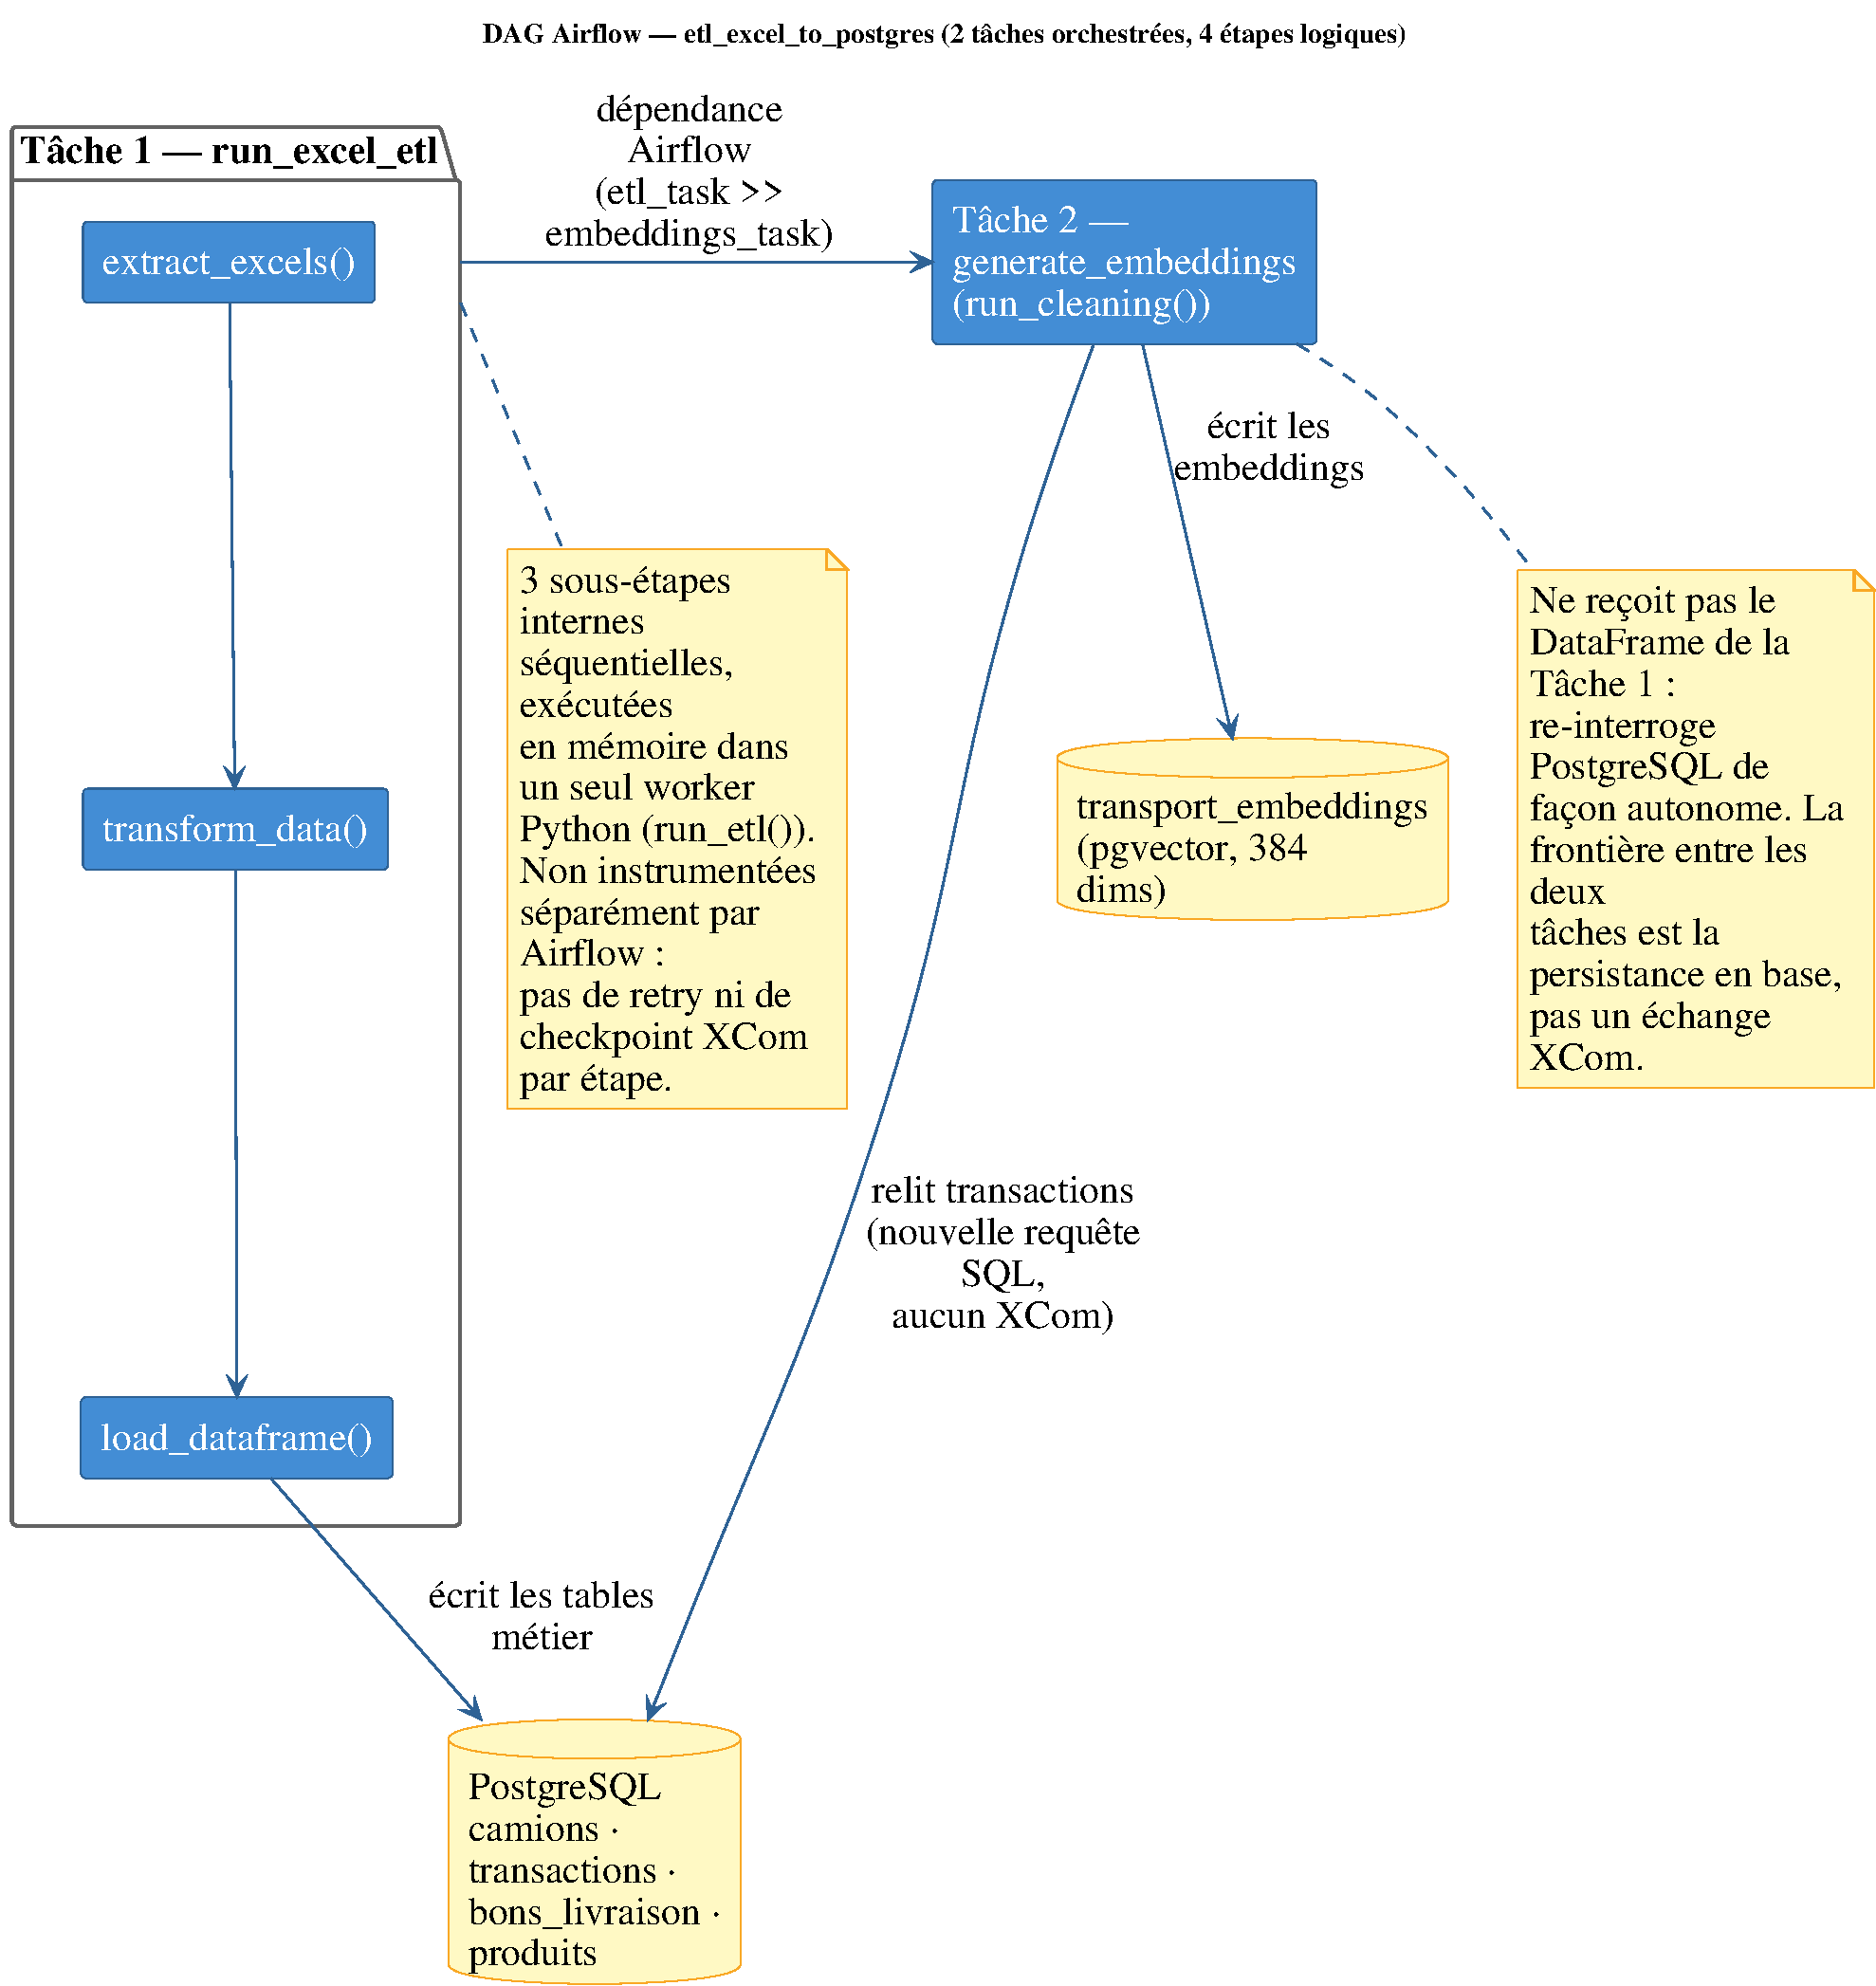
\includegraphics[width=\textwidth,height=0.88\textheight,keepaspectratio]{figures/fig_etl_dag.pdf}
    \caption{DAG Airflow \texttt{etl\_excel\_to\_postgres}, deux tâches orchestrées, quatre étapes logiques}
    \label{fig:etl_dag}
    \source{Schéma de l'auteur}
\end{figure}

\textbf{Pourquoi deux tâches, et pas quatre.} Découper extraction, transformation et chargement en trois tâches Airflow aurait obligé à faire transiter plusieurs milliers de lignes par \texttt{XCom}, un mécanisme qui n'est pas prévu pour ces volumes. Les regrouper garde les données en mémoire. Le prix est qu'un échec au chargement fait rejouer toute la tâche ; c'est sans danger, car l'extraction et la transformation sont rejouables à l'identique et le chargement est idempotent (\S\ref{sec: chargement}). La vectorisation, elle, est isolée pour une autre raison : c'est une charge de calcul, treize fois plus lente que le chargement (3~min~50 contre 17~s), qui mérite son propre suivi.

\textbf{Un déclenchement à la demande.} Les fichiers Excel contiennent des données personnelles : ils ne sont jamais versionnés, conformément à la loi n\textsuperscript{o}~2008-12 \cite{senegalLoi200812}. Un script transfère les fichiers vers le serveur par une liaison chiffrée, puis déclenche le DAG par l'API d'Airflow. Le DAG n'a donc pas de planification récurrente : il s'exécute à chaque dépôt de fichier.

\subsection{Extraction : absorber l'hétérogénéité des sources}
\label{sec: extraction}

L'informalité documentaire décrite dans l'état de l'art se lit dans chaque fichier. Les noms portent des doubles espaces ou un suffixe \texttt{- Copie} : aucune convention de nommage ne peut être présumée. Chaque feuille commence par une ligne de titre libre, suivie de deux lignes d'en-tête superposées. Les feuilles sont donc lues comme une grille brute, sans en-tête ; les noms de colonnes sont reconstitués à la transformation.

Les fichiers sont triés par ordre chronologique à partir du mois et de l'année lus dans leur nom. Un tri alphabétique placerait \textit{AOUT} avant \textit{AVRIL} et \textit{JANVIER}. Or la date d'émission d'un bon de livraison est fixée à sa première occurrence : sans ce tri, elle dépendrait de l'ordre des fichiers sur le disque, une corruption silencieuse. Chaque ligne est enfin étiquetée avec son fichier et sa feuille d'origine, pour l'audit et pour la clé de déduplication.

\subsection{Transformation et normalisation}
\label{sec: transformation}

\texttt{transform\_data()} impose un schéma unique en six étapes, chacune répondant à un défaut réel des classeurs :
\begin{enumerate}
    \item les deux lignes d'en-tête sont fusionnées en noms de colonnes (« Extrait » et « N° » deviennent \texttt{extrait\_n}) ;
    \item chaque colonne est reconnue par un motif sur son nom (\texttt{date}, \texttt{libell[eé]}, \texttt{camion}\ldots), et non par sa position, qui varie entre récapitulatifs mensuels et journaliers ; l'absence d'une colonne obligatoire arrête le traitement avec un message explicite ;
    \item les montants notés à la française (« 1.700.000 CFA ») sont convertis en nombres ;
    \item les dates sont lues au format jour/mois (\texttt{dayfirst=True}), sans quoi le 03/04 deviendrait le 4 mars ;
    \item les lignes « report solde », qui reportent un cumul d'une page à l'autre, sont écartées : elles fausseraient les totaux ;
    \item la clé de déduplication \texttt{source\_key} est calculée, après nettoyage, pour qu'un même montant écrit de deux façons produise la même clé.
\end{enumerate}

\subsection{Chargement idempotent}
\label{sec: chargement}

\textbf{La clé \texttt{source\_key}} est l'empreinte MD5 de neuf champs :
\[
\begin{aligned}
\texttt{source\_key} = \mathrm{MD5}\big(\;
  &\texttt{source\_file} \,\|\, \texttt{source\_sheet} \,\|\, \texttt{date\_transaction} \,\|\,{} \\
  &\texttt{libelle} \,\|\, \texttt{entrees\_appro} \,\|\, \texttt{sorties\_depenses} \,\|\,{} \\
  &\texttt{solde\_progressif} \,\|\, \texttt{camion\_raw} \,\|\, \texttt{bl\_raw}\;\big)
\end{aligned}
\]
Le fichier et la feuille séparent deux lignes identiques venues de mois différents ; le solde progressif, cumulatif, distingue deux lignes identiques d'un même fichier (plusieurs « CARBURANT GOLO » dans le mois). La colonne \texttt{source\_key} porte une contrainte d'unicité, et l'insertion utilise \texttt{ON CONFLICT (source\_key) DO NOTHING} : une ligne déjà présente est simplement comptée comme doublon. Rejouer le pipeline, entièrement ou en partie, n'insère donc aucun doublon ; c'est ce qui rend possible la reprise après une coupure de connexion (ADR-01).

\textbf{Des référentiels qui s'enrichissent.} Les tables \texttt{camions}, \texttt{bons\_livraison} et \texttt{produits} sont, elles, mises à jour à chaque import (\texttt{DO UPDATE}) : une transaction est un fait figé, un camion peut changer de statut. Un camion d'abord vu comme camion de la société peut être requalifié \texttt{particulier} par une « avance transport » ; l'inverse est interdit (Figure~\ref{fig:etl_table_camions}). Un libellé qui cite plusieurs camions est découpé et chaque camion est enregistré, mais seul le premier est rattaché à la transaction : c'est une limite du schéma. Une alerte signale les dépenses de carburant, de route, de ration ou d'amende sans camion identifié.

\begin{figure}[H]
    \centering
    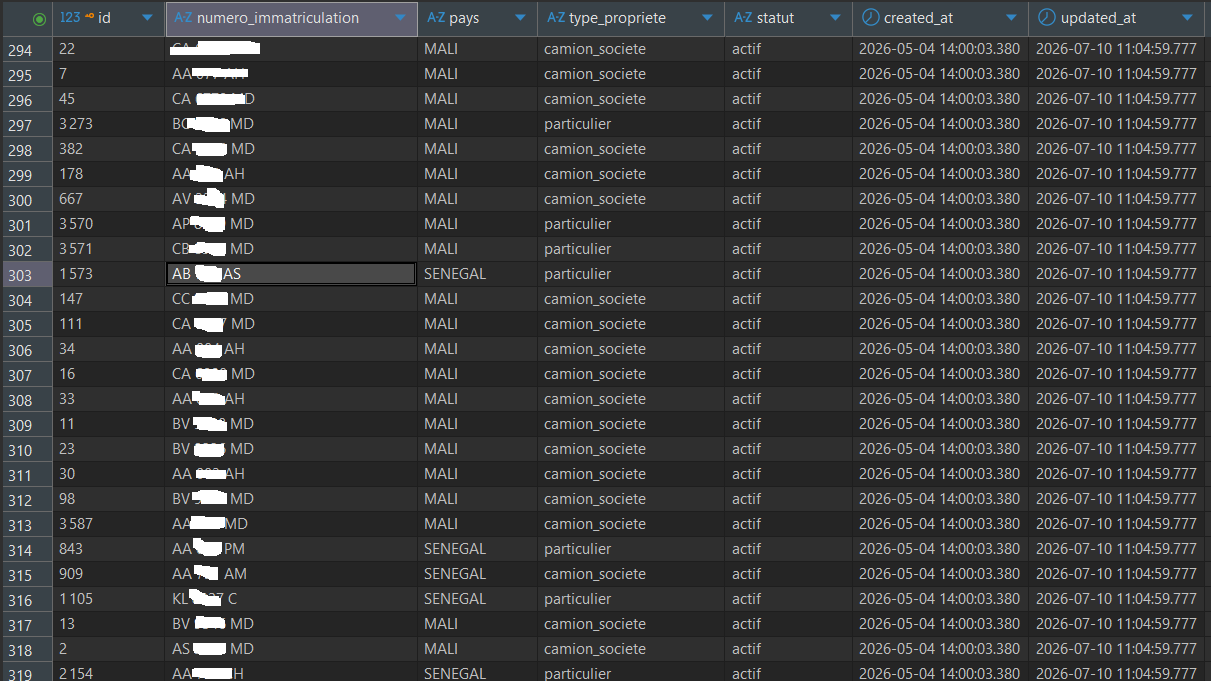
\includegraphics[width=0.8\textwidth]{figures/captures/etl_table_camions.png}
    \caption{Référentiel \texttt{camions} en base, classé par pays et type de propriété (extrait)}
    \label{fig:etl_table_camions}
\end{figure}

\begin{figure}[H]
    \centering
    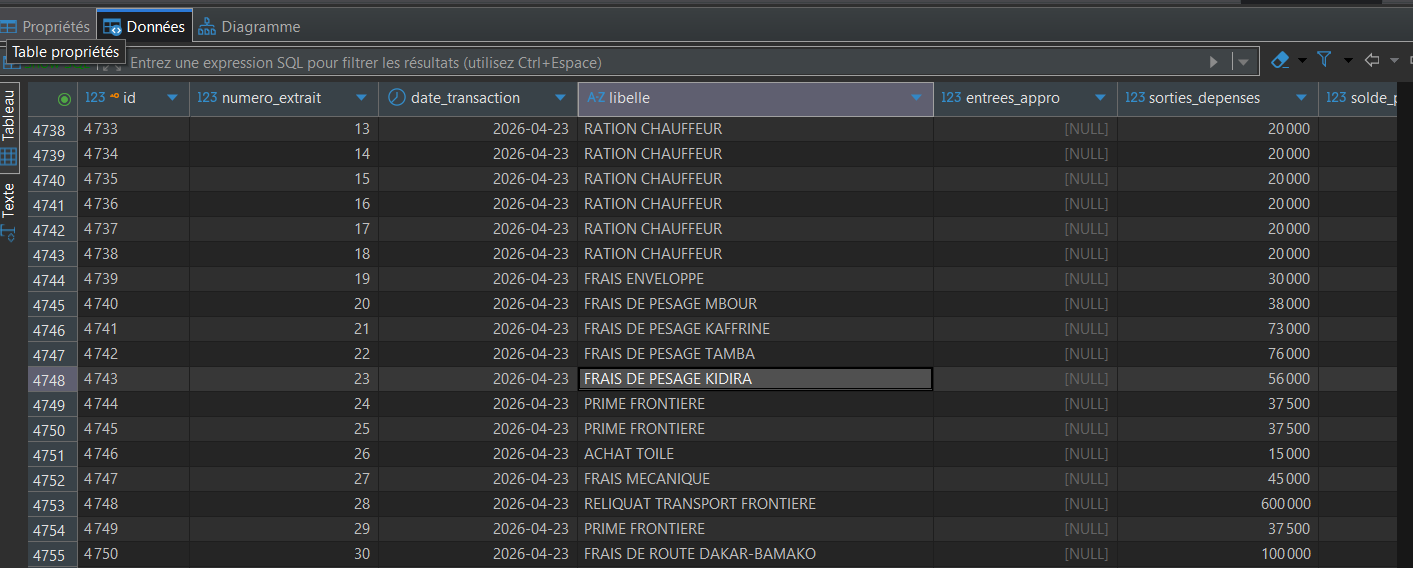
\includegraphics[width=0.8\textwidth]{figures/captures/etl_table_transactions.png}
    \caption{Transactions chargées dans PostgreSQL (extrait)}
    \label{fig:etl_table_transactions}
\end{figure}

\subsection{Vectorisation du batch ETL au corpus RAG}
\label{sec:  vectorisation}

La seconde tâche relit chaque transaction avec son camion, son bon de livraison et ses produits, compose un texte court (\textit{ex.} « Categorie carburant Camion AA~076~AH BL~1234 Produit gasoil »), puis le transforme en vecteur de 384 dimensions avec le modèle \texttt{all-MiniLM-L6-v2}. C'est le même modèle que celui qui encode les questions dans le service RAG local (\S\ref{sec:c4_composants}) : requêtes et corpus partagent le même espace. Les champs absents reçoivent une valeur explicite (\texttt{"inconnu"}) plutôt que la chaîne \texttt{"None"}. Les vecteurs sont enregistrés avec \texttt{ON CONFLICT (id) DO UPDATE} : rejouer la tâche rafraîchit les vecteurs sans les dupliquer (Figure~\ref{fig:etl_table_embeddings}).

\begin{figure}[H]
    \centering
    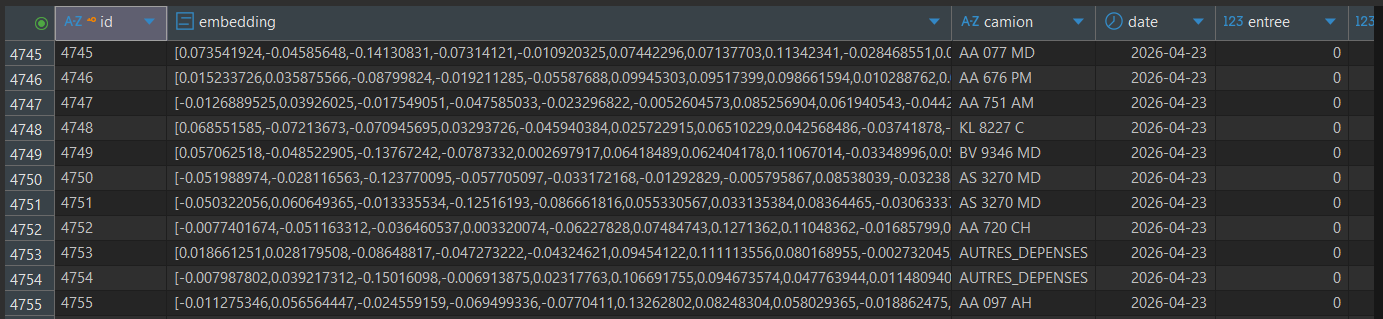
\includegraphics[width=0.8\textwidth]{figures/captures/etl_table_embeddings.png}
    \caption{Vecteurs d'embedding stockés dans \texttt{transport\_embeddings} (extrait)}
    \label{fig:etl_table_embeddings}
\end{figure}

\subsection{Validation du pipeline}
\label{sec: validation}

\textbf{Chargement initial.} Le 4~mai~2026, une exécution a ingéré 21 fichiers (15 récapitulatifs mensuels de janvier~2025 à mars~2026, 6 journaliers d'avril~2026). Elle a inséré 4~755 transactions, au-dessus du seuil de 4~500 de \texttt{ENF-VOL-01}. Les 3~595 enregistrements de camions correspondent à 319 camions distincts : un camion est compté à chaque apparition dans les transactions. Le Tableau~\ref{tab:validation_synthese} rassemble les chiffres.

\textbf{Preuve d'idempotence.} Le 10~juillet~2026, le même DAG a été relancé sur les mêmes fichiers, déjà chargés. Les deux tâches ont réussi (Figure~\ref{fig:etl_dag_rejeu}). Sur les 4~755 lignes, \textbf{4~755 ont été reconnues comme doublons et aucune n'a été insérée} (Figure~\ref{fig:etl_log_rejeu}). Les référentiels ont été mis à jour à l'identique. \texttt{EF-ETL-02} est ainsi démontrée par l'expérience, pas seulement par construction. La tâche de vectorisation compte 4~776 transactions : les 21 supplémentaires viennent de saisies de test faites dans l'application entre les deux dates (Figure~\ref{fig:etl_log_embeddings}).

\begin{figure}[H]
    \centering
    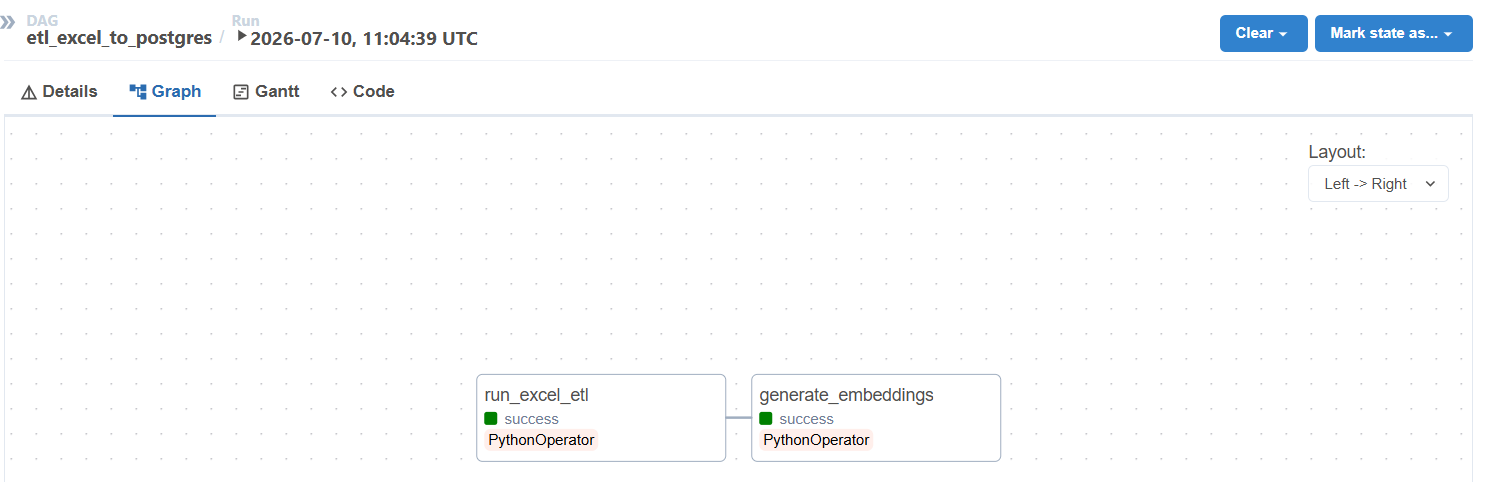
\includegraphics[width=0.8\textwidth]{figures/captures/etl_dag_rejeu.png}
    \caption{Rejeu de contrôle du 10~juillet~2026 dans Airflow : les deux tâches en succès}
    \label{fig:etl_dag_rejeu}
\end{figure}

\begin{figure}[H]
    \centering
    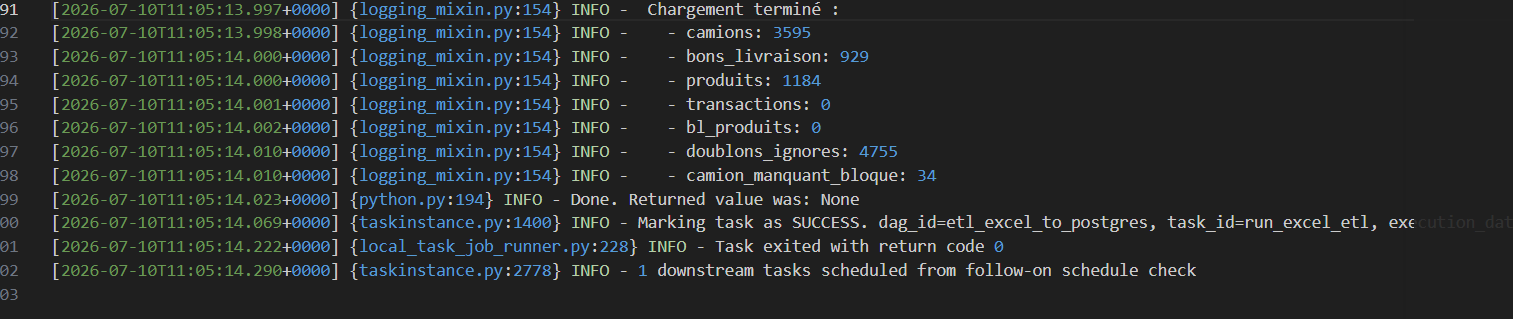
\includegraphics[width=0.95\textwidth]{figures/captures/etl_log_rejeu.png}
    \caption{Journal de la tâche \texttt{run\_excel\_etl} au rejeu : 0 transaction insérée, 4~755 doublons ignorés}
    \label{fig:etl_log_rejeu}
\end{figure}

\begin{figure}[H]
    \centering
    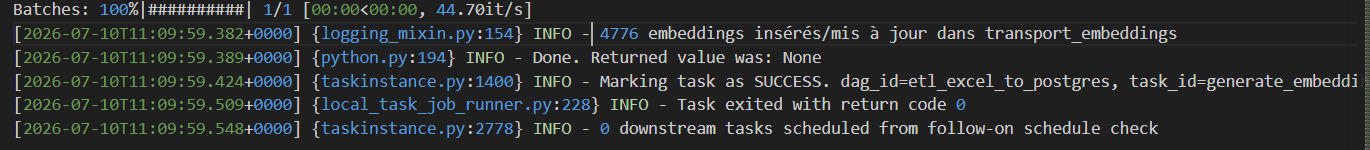
\includegraphics[width=0.95\textwidth]{figures/captures/etl_log_embeddings.png}
    \caption{Journal de la tâche \texttt{generate\_embeddings} au rejeu : 4~776 embeddings insérés ou mis à jour}
    \label{fig:etl_log_embeddings}
\end{figure}

\textbf{Rejets et durée.} L'extraction produit 5~023 lignes brutes ; 268 sont écartées (5,3~\%) : reports de solde, lignes sans date ou sans libellé, lignes de titre des fichiers suivant le premier. Le pipeline ne distingue pas ces causes : leur répartition n'est pas mesurée. Les 34 dépenses sans camion identifié sont chargées avec une alerte, pas rejetées. Le DAG complet s'exécute en moins de 4~min~35, ce qui permet un traitement après chaque dépôt de fichier.

\begin{table}[htbp]
\centering
\footnotesize
\caption{Validation du pipeline : chargement initial (04/05/2026) et rejeu de contrôle (10/07/2026)}
\label{tab:validation_synthese}
\begin{tabularx}{\linewidth}{|>{\raggedright\arraybackslash}X|>{\raggedright\arraybackslash}p{3.0cm}|>{\raggedright\arraybackslash}p{3.4cm}|}
\hline
\rowcolor[HTML]{EFEFEF}
\textbf{Métrique} & \textbf{Valeur mesurée} & \textbf{Exigence / statut} \\ \hline
Fichiers ingérés & 21 & \\ \hline
Transactions insérées & 4~755 & \texttt{ENF-VOL-01} ($\geq$~4~500) : dépassé \\ \hline
Camions : enregistrements / distincts & 3~595 / 319 & \\ \hline
Bons de livraison : enregistrements / distincts & 929 / 727 & \\ \hline
Produits : enregistrements / distincts & 1~184 / 633 & \\ \hline
Doublons reconnus au rejeu & 4~755 / 4~755 & \texttt{EF-ETL-02} : prouvé \\ \hline
Transactions insérées au rejeu & 0 & \texttt{EF-ETL-02} : prouvé \\ \hline
Lignes écartées & 268 / 5~023 (5,3~\%) & causes non ventilées \\ \hline
Dépenses sans camion identifié & 34 & chargées avec alerte \\ \hline
Durée : chargement / vectorisation / DAG & 17~s / 3~min~50 / 4~min~35 & \\ \hline
\end{tabularx}
\end{table}

\subsection{Synthèse et transition}
\label{sec: synthese-transition}

Le pipeline transforme des classeurs hétérogènes en une base relationnelle et vectorielle cohérente, qu'on peut rejouer sans risque. Il satisfait \texttt{EF-ETL-01}, \texttt{EF-ETL-02} et \texttt{ENF-VOL-01}. La section suivante décrit l'application web qui met ces données entre les mains des utilisateurs.
